\documentclass{VUMIFInfBakalaurinis}
\usepackage{algorithmicx}
\usepackage{algorithm}
\usepackage{algpseudocode}
\usepackage{amsfonts}
\usepackage{amsmath}
\usepackage{bm}
\usepackage{caption}
\usepackage{color}
\usepackage{float}
\usepackage{graphicx}
\usepackage{listings}
\usepackage{subfig}
\usepackage{url}
\usepackage{wrapfig}

\usepackage{longtable}
\usepackage{rotating}

\usepackage{amsbsy}

\usepackage{hyperref} %[pdfpagelabels,bookmarks,hyperindex,hyperfigures]

%\definecolor{mygray}{rgb}{0.5,0.5,0.5}
%\lstset{ %
%  numbers=left,                    	% where to put the line-numbers;
%  numbersep=5pt,                   	% how far the line-numbers are from the code
%  numberstyle=\tiny\color{mygray}, 	% the style that is used for the line-numbers 
%  breaklines=true,                 	% sets automatic line breaking
%  frame=single,	                   	% adds a frame around the code
%  morekeywords={of,in},				% if you want to add more keywords to the set
%  tabsize=2	                   		% sets default tabsize to 2 spaces
%}

%if errors .aux, .toc

\hypersetup{
    bookmarks=true,         % show bookmarks bar?
    %unicode=false,          % non-Latin characters in Acrobat’s bookmarks
    %pdftoolbar=true,        % show Acrobat’s toolbar?
    %pdfmenubar=true,        % show Acrobat’s menu?
    %pdffitwindow=false,     % window fit to page when opened
    %pdfstartview={FitH},    % fits the width of the page to the window
    pdftitle={Dalykinės srities modelio transformavimas į UML užduočių diagramas},    % title
    pdfauthor={Aleksandras Sivkovas},     % author
    hidelinks
}

%\definecolor{dkgreen}{rgb}{0,0.6,0}
%\definecolor{gray}{rgb}{0.5,0.5,0.5}
%\definecolor{mauve}{rgb}{0.58,0,0.82}
%\definecolor{light-gray}{gray}{0.25}
%keywordstyle=\bfseries\color{blue},
%  commentstyle=\itshape\color{dkgreen},
%  stringstyle=\color{mauve},

\lstdefinestyle{pseudocode}{
  language=Java,
  aboveskip=3mm,
  belowskip=3mm,
  showstringspaces=false,
  columns=flexible,
  basicstyle={\normalsize\ttfamily},
  numberstyle={\tiny},
  numbers=left,
  keywordstyle=\pmb,
  commentstyle=\itshape,
  stringstyle=\itshape,
  breaklines=true,
  breakatwhitespace=true,
  tabsize=2,
  morekeywords={of,in,function},
  escapeinside={(*}{*)},          % if you want to add LaTeX within your code
  frame=single	                   	% adds a frame around the code
}

%%% Table of contents to list down to subsections and no further
\setcounter{tocdepth}{4}
 
%%% Number down to subsubsections only
\setcounter{secnumdepth}{4}

% Titulinio aprašas
\university{Vilniaus universitetas}
\faculty{Matematikos ir informatikos fakultetas}
\department{Programų sistemų katedra}
\papertype{Baigiamasis bakalauro darbas}
\title{Dalykinės srities modelio transformavimas į UML užduočių diagramas}
\titleineng{Deriving use cases from business process}
\status{4 kurso 1 grupės studentas}
\author{Aleksandras Sivkovas}
% \secondauthor{Vardonis Pavardonis}   % Pridėti antrą autorių
\supervisor{Prof. dr. Saulius Gudas}
\reviewer{prof. habil. dr. Vardaitis Pavardaitis}
\date{Vilnius \\ \the\year}

% Nustatymai
% \setmainfont{Palemonas}   % Pakeisti teksto šriftą į Palemonas (turi būti įdiegtas sistemoje)
\bibliography{bibliografija} 

\begin{document}

\maketitle

\tableofcontents




%Įvade apibūdinamas darbo tikslas, temos aktualumas ir siekiami rezultatai.
\sectionnonum{Įvadas}

Reikalavimų inžinerija yra sudėtinga programų kūrimo dalis. Proceso sudėtingumas dažnai tampa klaidų priežastimi. Čia atsiradusios klaidos sunkiai aptinkamos ir sukelia brangiai kainuojančias pasekmes, nes sekančiuose etapuose bus kuriama neteisingai apibrėžta programa. Norint išvengti klaidų galima kai kurias proceso veiklas automatizuoti. Nors yra daug modeliavimo įrankių, juose trūksta automatinio vieno modelio generavimo iš kito.

Šio darbo tikslas – sukurti algoritmą \textbf{BPMN} modelio transformacijai į \textbf{užduočių diagramas} ir įgyvendinti programos prototipą. \textbf{Užduočių diagramos} yra svarbi reikalavimų inžinerijos dalis, kadangi ji apibrėžia naudotojo reikalavimus. Įmonės dažniausiai žino kaip ir kokias veiklas jos vykdo. Verslo procesą galima apibrėžti \textbf{BPMN} diagramomis. Bet ne viską, kas yra \textbf{BPMN} modelyje, galima perkelti į \textbf{užduočių diagramą}, todėl darbe bus apibrėžtas modifikuotas \textbf{BPMN} modelis, kuriame bus vaizduojama tik algoritmui aktuali informacija. Taip pat gali tekti pridėti papildomų atributų, kurie padės pasiekti tikslesnius rezultatus. Čia bus tiriamas \textbf{BPMN} modelio transformacijos į \textbf{užduočių diagramas} algoritmas.

Siekiami rezultatai yra:
\begin{enumerate}
	\item Algoritmas galintis transformuoti \textbf{BPMN} modelį į \textbf{užduočių diagramą}(angl. Use case diagram).
	\item Programa demonstruojanti algoritmo veikimą.
\end{enumerate}


%Pagrindinėje tiriamojoje dalyje aptariama ir pagrindžiama tyrimo metodika;
%pagal atitinkamas darbo dalis, nuosekliai, panaudojant lyginamosios analizės,
%klasifikacijos, sisteminimo metodus bei apibendrinimus, dėstoma sukaupta ir
%išanalizuota medžiaga. 
\section{BPMN diagrama}
\textbf{BPMN} specifikacija leidžia atvaizduoti gana nemažai verslo proceso atributų \cite{bpmnFormal}. Bet šiame darbe ji bus nagrinėjama tik kaip įvesties duomenų formatas, naudojamas apibrėžti informaciją pagal kurią bus kuriama \textbf{užduočių diagrama}. Taigi daugelį \textbf{BPMN} komponentų galima tiesiog ignoruoti, nes jie neturi jokios įtakos algoritmo vykdymo rezultatui. Norint pabrėžti svarbią informaciją, darbe bus tiriamos tik tos \textbf{BPMN} savybės kurios gali įtakoti algoritmo vykdymo rezultatą. Atitinkami komponentai pavaizduoti \ref{tab:investigated_bpmn_components} lentelėje.
\newcounter{counter:table:reset}
\newcounter{counter:table}[counter:table:reset]
\newcommand\rownumber{\stepcounter{counter:table}\arabic{counter:table}}
\begin{center}
    \begin{longtable}{ | p{0.5cm} | p{2cm} |  p{7cm} | p{4cm} |}
    \caption{BPMN diagramos komponentai}
	\label{tab:investigated_bpmn_components}
    \\ \hline 
    Nr. & Komponentas & Aprašymas & Žymėjimo pavizdys\\ 
    \hline 
    \rownumber & Juosta & Komponentas žymintis diagramos dalyvį ir nurodantis, kad jis atsakingas už veiklų esančių šiame komponente vykdymą. & \vtop{\hbox{\strut }\hbox{\strut 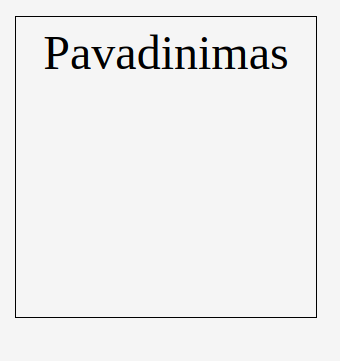
\includegraphics[width=3cm]{img/bpm-components/pool}}} \\
    \hline
     \rownumber & Įvykis & Komponentas žymintis, kad ivyko kažkas kas įtakojo proceso būseną. & \vtop{\hbox{\strut }\hbox{\strut 
\includegraphics[width=3cm]{img/bpm-components/event}}} \\ 
    \hline 
    \rownumber & Veikla & Komponentas žymintis užduoties vykdymo procesą & \vtop{\hbox{\strut }\hbox{\strut 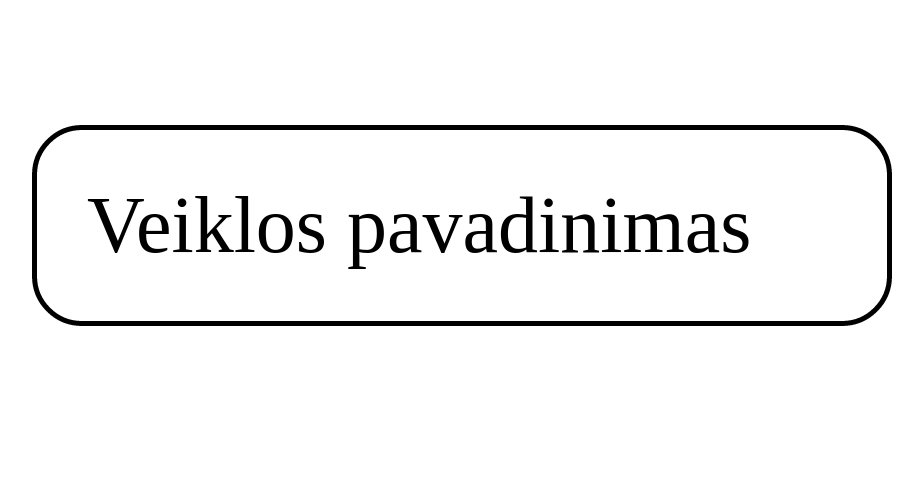
\includegraphics[width=3cm]{img/bpm-components/activity}}}\\
    \hline 
    \rownumber & Sekos srautas & Komponentas žymintis veiklų seką. & \vtop{\hbox{\strut }\hbox{\strut 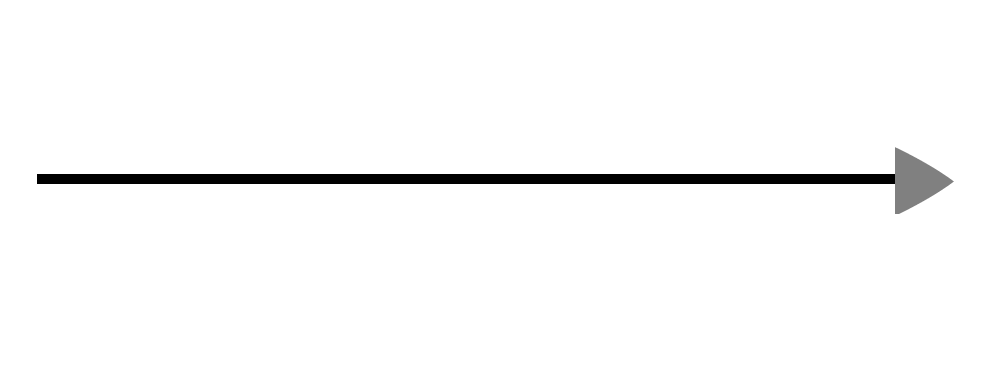
\includegraphics[width=3cm]{img/bpm-components/transition}}}\\
    \hline
    \rownumber & Transakcija & Subprocesas kuris užtikrina, kad veiklos jame būtų pilnai įvykdytos arba atšauktos. & \vtop{\hbox{\strut }\hbox{\strut 
\includegraphics[width=3cm]{img/bpm-components/transaction}}}\\
    \hline
%    \rownumber & Duomenų objektas & Komponentas žymintis sukuriamus arba įeities duomenis. & \vtop{\hbox{\strut }\hbox{\strut 
\includegraphics[width=3cm]{img/bpm-components/data_object}}}\\
%    \hline
%    \rownumber & Pranešimų srautas & Komponentas žymintis duomenų apsikeitimo srautus. & \vtop{\hbox{\strut }\hbox{\strut 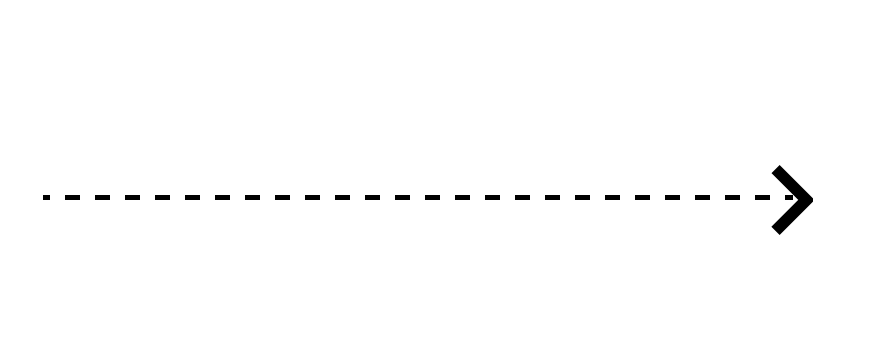
\includegraphics[width=3cm]{img/bpm-components/message_flow}}}\\
%    \hline
%    \rownumber & Sprendimas & Komponentas žymintis sekos srautų išsišakojimą. & \vtop{\hbox{\strut }\hbox{\strut 
\includegraphics[width=3cm]{img/bpm-components/gateway}}}\\
%    \hline
    \end{longtable}
\end{center}

Darbe bus nagrinėjamas procesas kuriam modeliuojama programų sistema, todėl materialios  veiklos bus atskirtos nuo duomenų tvarkymo veiklų \cite{bpmnPorterModel}. \textbf{BPMN} diagrama bus vaizduojama kaip detalizuotas M. Porterio vertės grandinės modelis (\ref{img:detalized_porter_vcm} pav), todėl į apibrėžimą įtrauktas sprendimas, kuris bus naudojamas išsišakojimui pavaizduoti. Tokiu būdu dėmesys telkiamas ties informacijos procesais.

\begin{figure}[H]
	\centering
	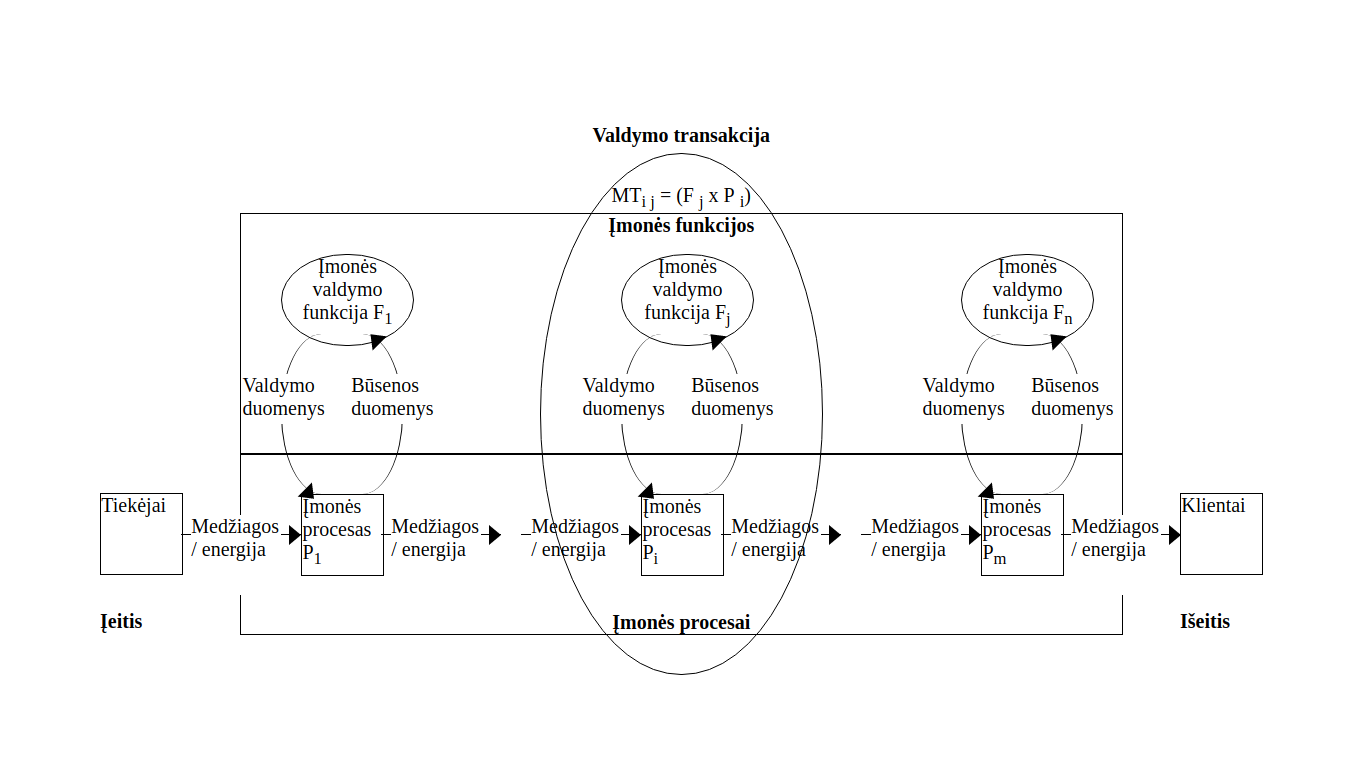
\includegraphics[width=\textwidth]{img/detalized_porter_vcm}
	\caption{Detalizuotas M. Porterio vertės grandinės modelis}
	\label{img:detalized_porter_vcm}
\end{figure} 


\section{Užduočių diagrama}

Čia pateikiamas \textbf{užduočių diagramos} naudojamos darbe apibrėžimas. Tai bus algoritmo rezultato formatas. Siekiama gauti kiek įmanoma tikslesnę užduočių diagramą. Jos komponentai pateikiam \ref{tab:investigated_use_case_diagram_components} lentelėje.
\stepcounter{counter:table:reset}
\begin{center}
    \begin{longtable}{ | p{0.5cm} | p{2cm} |  p{7cm} | c |}
    \caption{\textbf{Užduočių diagramos} komponentai}
	\label{tab:investigated_use_case_diagram_components}
    \\ \hline 
    Nr. & Komponentas & Aprašymas & Žymėjimo pavizdys\\ 
    \hline 
    \rownumber & Aktorius & Komponentas žymintis sistemos naudotojo tipą. & \vtop{\hbox{\strut }\hbox{\strut 
\includegraphics[width=3cm]{img/use_case_components/actor}}} \\
    \hline
    \rownumber & Vartojimo atvejis & Komponentas specifikuojantis elgsenų aibę, kuri generuoja rezultatą. & \vtop{\hbox{\strut }\hbox{\strut 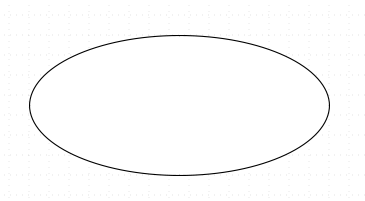
\includegraphics[height=3cm]{img/use_case_components/use_case}}} \\
    \hline
     \rownumber & Asociacija & Komponentas žymintis ryšį tarp aktoriaus ir vartojimo atvejo. & \vtop{\hbox{\strut }\hbox{\strut 
\includegraphics[width=3cm]{img/use_case_components/association}}} \\
    \hline
     \rownumber & Įtraukia & Komponentas žymintis elgseną kuri yra bendra keliems vartojimo atvejams, todėl ji parodoma atskirai nuo jų, kad būtų galima perpanaudoti. & \vtop{\hbox{\strut }\hbox{\strut 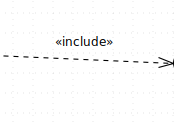
\includegraphics[width=3cm]{img/use_case_components/includes}}} \\
    \hline
    \rownumber & Išplečia & Komponentas žymintis, kad esant tam tikram atvejui vartojimo atvejis įtraukia papildomus vartojimo atvejus. & \vtop{\hbox{\strut }\hbox{\strut 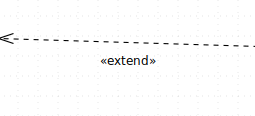
\includegraphics[width=3cm]{img/use_case_components/extend}}} \\
    \hline
    \end{longtable}
\end{center}

\section{\textbf{UML} diagramų transformavimo algoritmai}
\subsection{ Algoritmas \textbf{BPMN} modeliui transformuoti į \textbf{Užduočių diagramą}} \label{section:use_cases_from_bpmn}
Literatųroje yra parašyta apie \textbf{vartojimo atvejų diagramos} išvedimą iš \textbf{BPMN} modelio \cite{algUseCasesFromBpmn}. Straipsnyje aprašytas algoritmas atlieka (\ref{eq:use_cases_from_bpmn}) transformaciją. Imamas modifikuotas \textbf{BPMN} modelis (\ref{eq:use_cases_from_bpmn:bpmn_elements}) ir tie \textbf{vartojimo atvejų diagramos} komponentai, kurie gali būti iš jo išvesti (\ref{eq:use_cases_from_bpmn:use_case_elements}). 
\begin{align}
&BPMNElements = \left\{Start,End,Role,Branch,Task,Transition\right\}; \label{eq:use_cases_from_bpmn:bpmn_elements} \\
\begin{split}
&UseCasesElements = \left\{Actor, Generalization, Association,Use Case,\right. \\
&\left. Include, Extension Point, Extend\right\}; \label{eq:use_cases_from_bpmn:use_case_elements}\\
\end{split} \\
&BPMN(BPMNModelElements) \Rightarrow UseCases(UseCasesElements); \label{eq:use_cases_from_bpmn}
\end{align}

Algoritmo autoriai pirmiausia siūlo surasti ryšius tarp modelių. Juostos atitinka aktorius. Užduotys tuo tarpu grupuojamos, kol nepasiekia maksimalaus skaičiaus vykdomų be pertraukos, priklausančių tai pačiai juostai ir pagaminančių rezultatą. Tokia grupė pavadinama žingsniu ir yra laikoma atitinkančia vartojimo atvejį.  Tuomet lieka surasti kaip dar galima būtų panaudoti informaciją, patikslinti ir suprastinti gautoms diagramoms.

Vėliau pristatomas algoritmas. Jis Pirmiausia sudėlioja užduotis į proceso žingsnius. Vėliau juostos tampa aktoriais, o žingsniai jose – vartojimo atvejais. Galiausiai pasikartojančios užduotis išimamos iš žingsnių ir prijungiamos asociacija įtraukia arba išplečia pagal situaciją.

\section{\textbf{Užduočių diagramos} išvedimas iš \textbf{BPMN} modelio}

Šio darbo tikslas, algoritmas galintis gauti \textbf{užduočių diagramas} iš \textbf{BPMN} modelio, bus kuriamas pagal \ref{section:use_cases_from_bpmn} aprašytą algoritmo sukūrimo pavyzdį. Pirmiausia bus rasti ryšiai tarp diagramų, vėliau sukurtas būdas juos panaudoti, galiausiai panaudota likusi modelio informacija patikslinti ir suprastinti diagramoms.

\subsection{Ryšiai tarp \textbf{BPMN} ir \textbf{užduočių diagramų}} \label{section:relations_sd_bpmn}

Norint duomenis iš vieno modelio perkelti į kitą galima pasinaudoti ryšiais esančiais tarp jų.

\begin{center}
    \begin{longtable}{ | c | c |  c | c | c | c |}
    \caption{Ryšiai tarp \textbf{BPMN} ir \textbf{užduočių diagramų}}
	\label{tab:relations_sd_bpmn}
    \\ \hline 
     & 
     %\begin{turn}{-90}
     Aktorius 
     %\end{turn} 
     & 
     %\begin{turn}{-90}
     Vartojimo atvejis 
     %\end{turn}  
     & 
     %\begin{turn}{-90}
     Asociacija 
     %\end{turn}  
     & 
     %\begin{turn}{-90}
     Įtraukia 
     %\end{turn} 
     & 
     %\begin{turn}{-90}
     Išplečia 
     %\end{turn} 
     \\ 
    \hline 
    Juosta & + & & + &  &  \\
    \hline
    Veikla  & & + & + & + & + \\
    \hline
    Transakcija & & + & & + & + \\
    \hline
    Sekos srautas  & &  & & & \\
    \hline
    Įvykis  & & & & & \\
    \hline 
    Duomenų objektas  & & & & & \\
    \hline
    Pranešimų srautas  & & & & & \\
    \hline
    Sprendimas  & & & & & \\
    \hline
    \end{longtable}
\end{center} 

\begin{enumerate}
	\item Aktorius – galima gauti iš informacijos esančios juostoje. 
	\item Vartojimo atvejis – gaunamas iš informacijos veiklose arba transakcijose. Vartojimo atvejis paprastai yra transakcijos tipo.
	\item Asociacija – ryšys tarp juostos ir veiklų joje.
	\item Įtraukia – veiklos kurias apima transakcija.
	\item Išplečia – ryšys randamas kai veikla pasikartoja skirtingose transakcijose.
\end{enumerate} 

Rasti ryšiai taip pat parodo kurie komponentai bus imami ir kurie gaunami. Taigi galima apibrėžti algoritmo įvesties ir išvesties duomenis.

%Citavimo pavyzdžiai: cituojamas vienas šaltinis \cite{PvzStraipsnLt}; cituojami
%keli šaltiniai \cite{PvzStraipsnEn, PvzKonfLt, PvzKonfEn, PvzKnygLt, PvzKnygEn,
%PvzElPubLt, PvzElPubEn, PvzMagistrLt, PvzPhdEn}.

\subsection{Ryšių tarp diagramų panaudojimas transformacijai}

Rasti ryšiai parodo į kokius \textbf{BPMN} komponentus reikia žiūrėti išvedant \textbf{užduočių diagramos} dalis. Toliau peržiūrimi diagramos variantai ir sudėliojami konkretūs žingsniai kuriuos reikia atlikti. Galiausiai gaunamas pseudokodas (Pseudokodas \ref{lst:bpmn_to_uc_pseudocode}). Jo veikimas pažingsniui aprašomas, taip pat pavaizduotas (pav. \ref{img:algorythm_activity_diagram}).

\begin{figure}[H]
	\centering
	\caption{Algoritmo diagrama}
	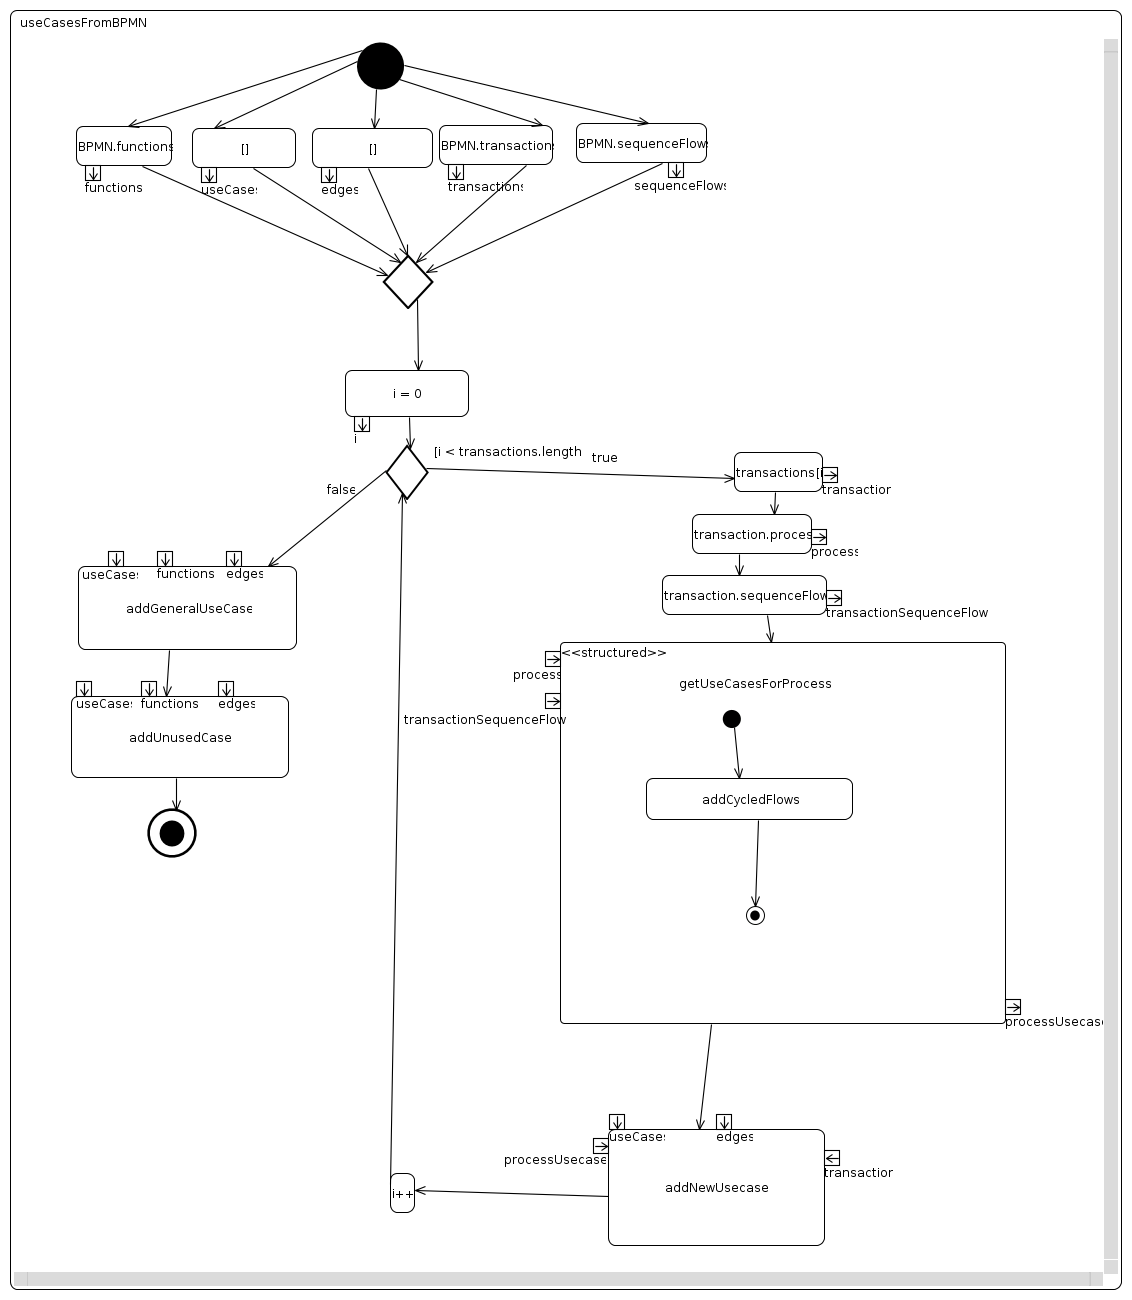
\includegraphics[scale=0.5]{img/algorythm-activity-diagram}
	\label{img:algorythm_activity_diagram}
\end{figure} 

\renewcommand{\lstlistingname}{Pseudokodas}% Listing -> Algorithm
\renewcommand{\lstlistlistingname}{Pseudokodo fragmentai}% List of Listings -> List of Algorithms
\begin{enumerate}
	\item Iškviečiama funkcija useCasesFromBPMN (Pseudokodas \ref{lst:bpmn_to_uc_pseudocode}) paduodant jai \textbf{BPMN} modelį.
	\lstinputlisting[style=pseudocode, caption={\textbf{UML} \textbf{Užduočių diagramos} gavimo iš \textbf{BPMN} modelio algoritmo pseudokodas}, label={lst:bpmn_to_uc_pseudocode}]{algorythm-pseudocode/useCasesFromBPMN}
	\item Po duomenų inicializavimo pirmiausia imamas transakcijos procesas (eil. \ref{line:bpmn_to_uc_pseudocode_get_process}) ir gaunami sekos srautai jungiantys komponentus transakcijoje (eil. \ref{line:bpmn_to_uc_pseudocode_get_transactionSequenceFlows}). 
	\item Vėliau sukuriami vartojimo atvejai apibrėžiantys proceso valdymą (eil. \ref{line:bpmn_to_uc_pseudocode_get_processUsecases}) funkcija getUseCasesForProcess (Pseudokodas  \ref{lst:bpmn_to_uc_pseudocode_getUseCasesForProcess}).
	\lstinputlisting[style=pseudocode, caption={Funkcija getUseCasesForProcess}, label={lst:bpmn_to_uc_pseudocode_getUseCasesForProcess}]{algorythm-pseudocode/getUseCasesForProcess}
	\item Joje randami sekos srautai išeinantys iš proceso (eil. \ref{line:bpmn_to_uc_pseudocode_getUseCasesForProcess_get_processFlows}) ir kiekvienam iš jų rekursijos būdu surandami ciklai su procesu funkcija addCycledFlows (Pseudokodas  \ref{lst:bpmn_to_uc_pseudocode_addCycledFlows}). Kiekvienam iš cikle esančių sekos srautų sukuriamas vartojimo atvejis (eil. \ref{line:bpmn_to_uc_pseudocode_getUseCasesForProcess_get_processUsecases_begin} - \ref{line:bpmn_to_uc_pseudocode_getUseCasesForProcess_get_processUsecases_end}). Jų kolekcija ir yra (Pseudokodas  \ref{lst:bpmn_to_uc_pseudocode_getUseCasesForProcess}) grąžinamas rezultatas.
	\lstinputlisting[style=pseudocode, caption={Funkcija addCycledFlows}, label={lst:bpmn_to_uc_pseudocode_addCycledFlows}]{algorythm-pseudocode/addCycledFlows}
Minėta Funkcija (Pseudokodas  \ref{lst:bpmn_to_uc_pseudocode_addCycledFlows}) pirmiausia patikrina ar jau nėra ciklo su procesu ir jei taip patvirtina, kad parametras currentPath turi savyje kelia į procesą (eil. \ref{line:bpmn_to_uc_pseudocode_addCycledFlows_isTargetProcess_begin} - \ref{line:bpmn_to_uc_pseudocode_addCycledFlows_isTargetProcess_end}). Jei kelias užsiciklino grąžinamas neigiamas atsakymas (eil. \ref{line:bpmn_to_uc_pseudocode_addCycledFlows_isGoingInCircles_begin} - \ref{line:bpmn_to_uc_pseudocode_addCycledFlows_isGoingInCircles_end}), tai reiškia grįžimą atgal. Jei žingsnis veda į jau išsaugotą sėkmingą kelio atkarpą patvirtinamas jo teisingumas (eil. \ref{line:bpmn_to_uc_pseudocode_addCycledFlows_isAlreadyFound_begin} - \ref{line:bpmn_to_uc_pseudocode_addCycledFlows_isAlreadyFound_end}). Jei nei viena iš šių sąlygų nepasitvirtino paimami sekantys žingsniai  (eil. \ref{line:bpmn_to_uc_pseudocode_addCycledFlows_getNextFlows}). Jų neradus pranešama apie aklavietę (eil. \ref{line:bpmn_to_uc_pseudocode_addCycledFlows_isDeadEnd_begin} - \ref{line:bpmn_to_uc_pseudocode_addCycledFlows_isDeadEnd_end}). Kol kas pažymima, kad žingsnis yra sėkmingas (eil. \ref{line:bpmn_to_uc_pseudocode_addCycledFlows_soFarSoGood}) ir žengtas (eil. \ref{line:bpmn_to_uc_pseudocode_addCycledFlows_takeStep}). Toliau ieškoma ciklų su procesu einant sekančiais sekos srautais (eil.  \ref{line:bpmn_to_uc_pseudocode_addCycledFlows_continueRecursion_begin} - \ref{line:bpmn_to_uc_pseudocode_addCycledFlows_continueRecursion_end}). Neradus nei vieno kelio į procesą ištrinamas pažymėjimas apie žingsnio teisingumą (eil.  \ref{line:bpmn_to_uc_pseudocode_addCycledFlows_isPathFound_begin} - \ref{line:bpmn_to_uc_pseudocode_addCycledFlows_isPathFound_end}). Kadangi keliai žengus šį žingsnį ištyrinėti grįžtama atgal (eil. \ref{line:bpmn_to_uc_pseudocode_addCycledFlows_stepBack}).
	\item (Pseudokodas \ref{lst:bpmn_to_uc_pseudocode_getUseCasesForProcess}) sukurti vartojimo atvejai pridedami prie jau gautų vartojimo atvejų kartu su ryšiais tarp jų funkcija addNewUsecases (Pseudokodas  \ref{lst:bpmn_to_uc_pseudocode_addNewUsecases}). 
\lstinputlisting[style=pseudocode, caption={Funkcija addNewUsecases}, label={lst:bpmn_to_uc_pseudocode_addNewUsecases}]{algorythm-pseudocode/addNewUsecases}	
Joje sukuriamas vartojimo atvejis visai transakcijai (eil. \ref{line:bpmn_to_uc_pseudocode_addNewUsecases_transactionUseCase}), pažiūrima kiek vartojimo atvejų rasta, jei vienas tai jo informacija išsaugoma į pagrindinį vartojimo atvejį (eil.  \ref{line:bpmn_to_uc_pseudocode_addNewUsecases_onlyMain_begin} - \ref{line:bpmn_to_uc_pseudocode_addNewUsecases_onlyMain_end}). Radus daugiau, jie išsaugomi kaip įeinantys į transakciją (eil.  \ref{line:bpmn_to_uc_pseudocode_addNewUsecases_addIncluded_begin} - \ref{line:bpmn_to_uc_pseudocode_addNewUsecases_addIncluded_end}). 
	\item Galiausiai randamos bendros funkcijos tarp transakcijų ir sukuriami apibendrinantys vartojimo atvejai (Pseudokodas  \ref{lst:bpmn_to_uc_pseudocode_addGeneralUseCases}).
	\lstinputlisting[style=pseudocode, caption={Funkcija addGeneralUseCases}, label={lst:bpmn_to_uc_pseudocode_addGeneralUseCases}]{algorythm-pseudocode/addGeneralUseCases}
	\item Jeigu liko nepanaudotų funkcijų, iš jų sukuriami vartojimo atvejai su perspėjimais (Pseudokodas \ref{lst:bpmn_to_uc_pseudocode_addUnusedCases}).
	\lstinputlisting[style=pseudocode, caption={Funkcija addUnusedCases}, label={lst:bpmn_to_uc_pseudocode_addUnusedCases}]{algorythm-pseudocode/addUnusedCases}
\end{enumerate} 

Atlikusi šio algoritmo veiksmus programa iš \ref{appendix:dvcm_window} priede pavaizduoto vertės grandinės modelio gauna \ref{appendix:use_cases_window} priede pavaizduotą \textbf{užduočių diagramą}.

%Iš diagramos \ref{img:bpmn} gaunama diagrama \ref{img:sequence}.

%\begin{figure}[H]
%	\centering
%	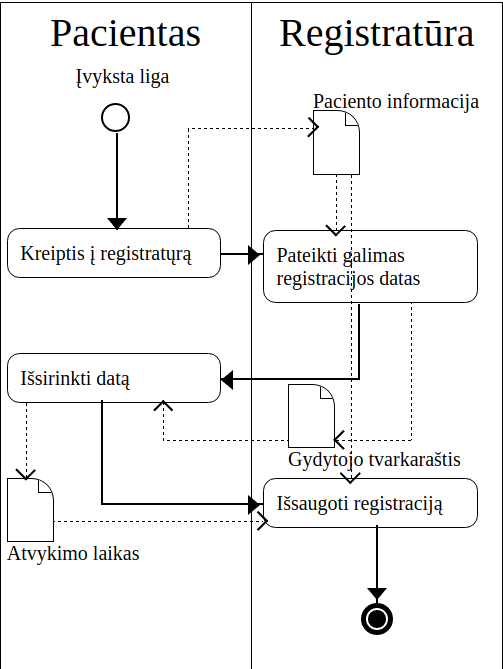
\includegraphics[scale=0.5]{img/bpmn_diagrama}
%	\caption{\textbf{BPMN} diagrama}
%	\label{img:bpmn}
%\end{figure} 
%\begin{figure}[H]
%	\centering
%	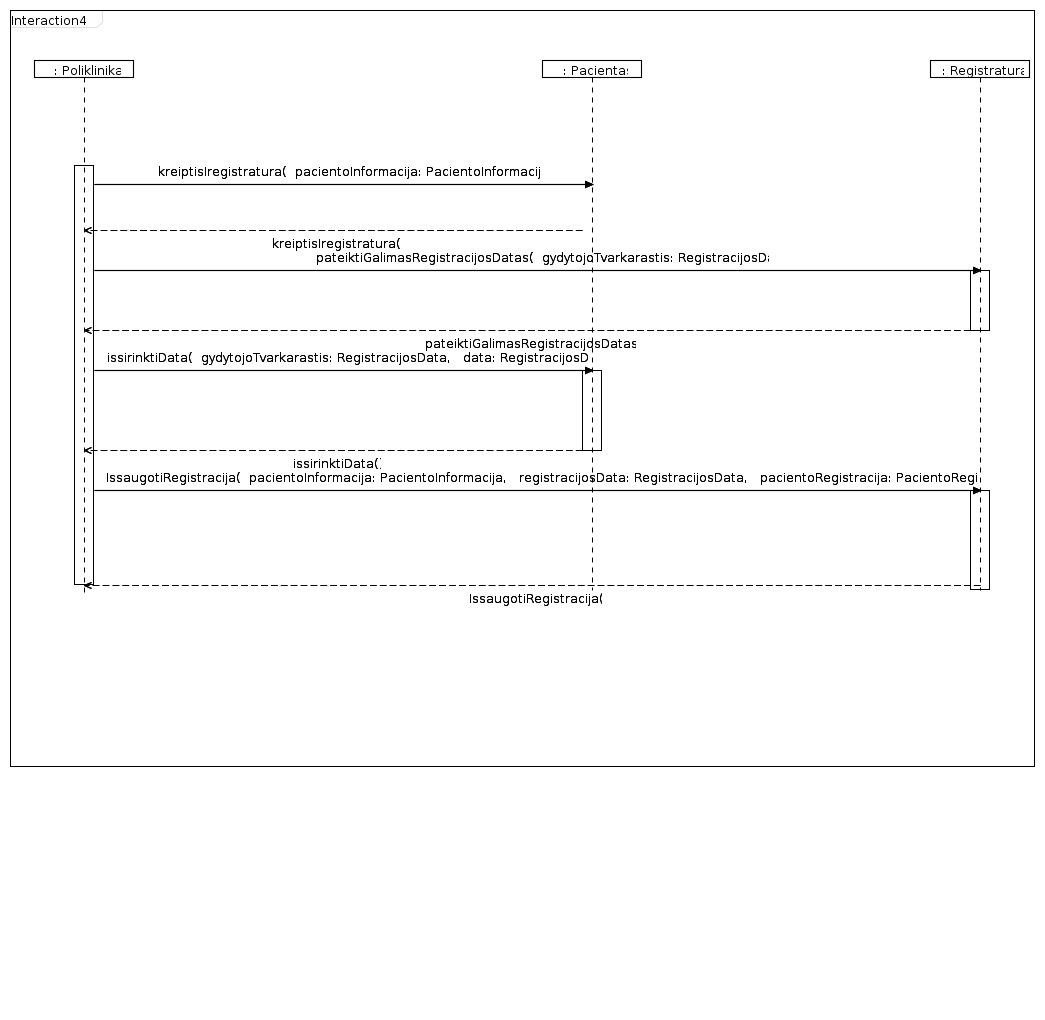
\includegraphics[scale=0.5]{img/sequence_example}
%	\caption{\textbf{užduočių diagramą} diagrama}
%	\label{img:sequence}
%\end{figure} 

%\subsection{Likusios informacijos panaudojimas suprastinti ar patikslinti diagramai}


\section{Programa \textbf{BPMN} transformacijai į \textbf{užduočių diagramą}}   


%Išvadose ir pasiūlymuose, nekartojant atskirų dalių apibendrinimų,
%suformuluojamos svarbiausios darbo išvados, rekomendacijos bei pasiūlymai.
\sectionnonum{Išvados}

%Šiame skyriuje pateikiamos išvados (reziume) anglų kalba.
\sectionnonum{Conclusions}


% bibliografija.bib faile. Šaltinių sąraše nurodoma panaudota literatūra,
% kitokie šaltiniai. Abėcėlės tvarka išdėstoma tik darbe panaudotų (cituotų,
% perfrazuotų ar bent paminėtų) mokslo leidinių, kitokių publikacijų
% bibliografiniai aprašai (šiuo punktu pasirūpina LaTeX). Aprašai pateikiami
% netransliteruoti.
\printbibliography[heading=bibintoc] % Literatūros šaltiniai aprašomi

\sectionnonum{Santrumpos}
Šiame darbe naudojami žymėjimai:
\begin{enumerate}
	\item \textbf{BPMN} – modeliavimo kalba, skirta pavaizduoti informaciją plačiai auditorijai. \textbf{BPMN} buvo sukurta ir dažniausia naudojama pavaizduoti verslo procesams \cite{bpmnFormal}.
	\item \textbf{UML} – modeliavimo kalba, skirta suteikti standartinį sistemos analizės, architektūros, veikimo ir kūrimo pavaizdavimą \cite{omgUmlFormal}.
	\item \textbf{Sekų diagrama} (angl. sequence diagram) – \textbf{UML} diagrama, skirta pavaizduoti žinučių tarp apibrėžtų objektų sekai tų objektų gyvavimo metu \cite{omgUmlFormal}.
	\item \textbf{Užduočių diagrama} (angl. use case diagram) – \textbf{UML} diagrama, skirta pavaizduoti pavaizduoti kaip gali būti naudojama programų sistema \cite{algUseCasesFromBpmn}.
\end{enumerate}

% Prieduose gali būti pateikiama pagalbinė, ypač darbo autoriaus savarankiškai
% parengta, medžiaga. Savarankiški priedai gali būti pateikiami kompiuterio
% diskelyje ar kompaktiniame diske. Priedai taip pat vadinami ir numeruojami.
% Tekstas su priedais siejamas nuorodomis (pvz.: \ref{img:mlp}).
\appendix  % Priedai


\section{Vertės grandinės modelis programos lange} \label{appendix:dvcm_window}
\begin{figure}[H]
    \centering
    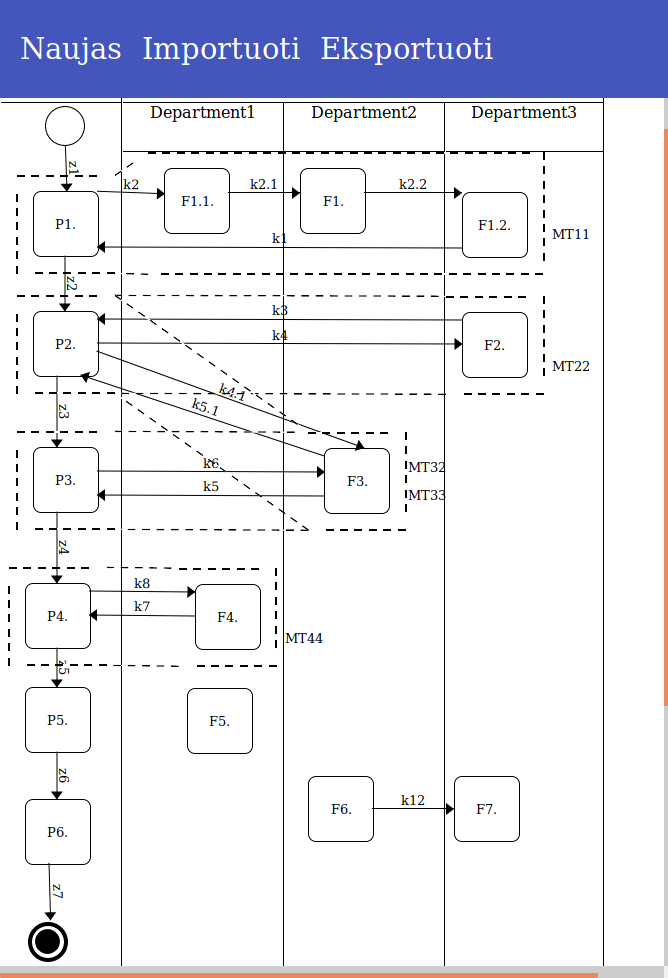
\includegraphics[scale=0.6]{img/dvcm_window}
%    \caption{Paveikslėlio pavyzdys}
%    \label{img:dvcm_window}
\end{figure}
\section{Transformuotas užduočių diagrama programos lange} \label{appendix:use_cases_window}
\begin{figure}[H]
    \centering
    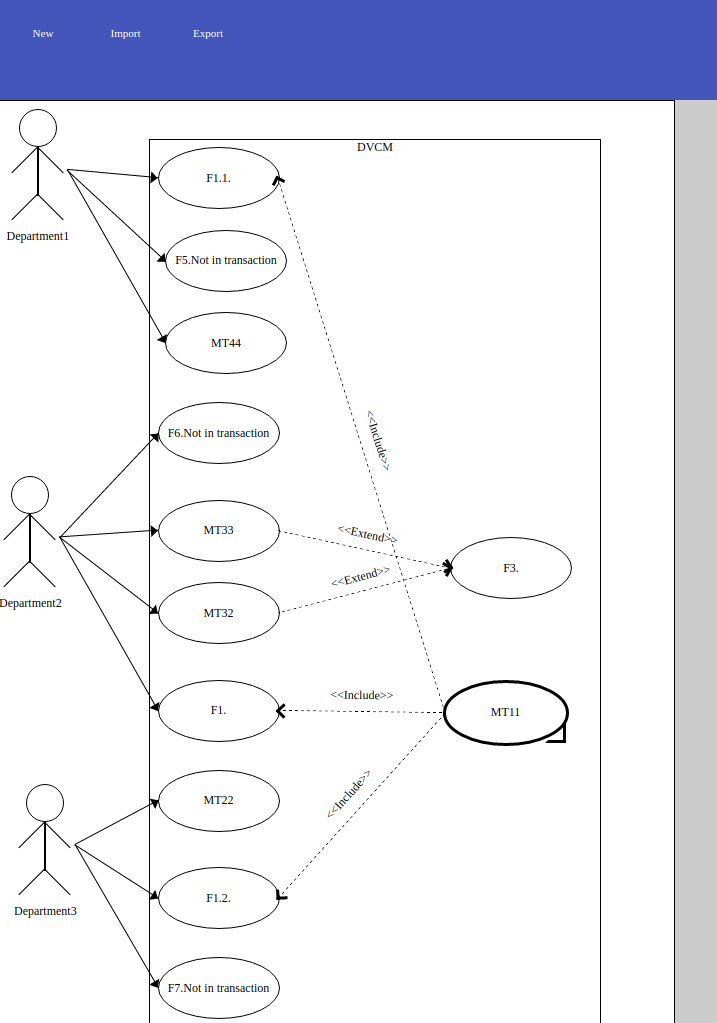
\includegraphics[scale=0.6]{img/use_cases_window}
%    \caption{Paveikslėlio pavyzdys}
%    \label{img:use_cases_window}
\end{figure}

%\section{Eksperimentinio palyginimo rezultatai}
% tablesgenerator.com - converts calculators (e.g. excel) tables to LaTeX
%\begin{table}[H]\footnotesize
%  \centering
%  \caption{Lentelės pavyzdys}
%  {\begin{tabular}{|l|c|c|} \hline
%    Algoritmas & $\bar{x}$ & $\sigma^{2}$ \\
%    \hline
%    Algoritmas A  & 1.6335    & 0.5584       \\
%    Algoritmas B  & 1.7395    & 0.5647       \\
%    \hline
%  \end{tabular}}
%  \label{tab:table example}
%\end{table}
\end{document}
